\documentclass[11pt,a4paper]{article}
\usepackage[margin=2.3cm]{geometry}
\usepackage{amsmath,amssymb}
\usepackage{booktabs}
\usepackage{graphicx}
\usepackage{hyperref}
\usepackage{float}
\usepackage{tikz}
\usetikzlibrary{arrows.meta,positioning}

\title{Resumen del paper y aplicacion al proyecto\\
\large Gradient pathologies en PINNs para difusion de calor 1D}
\author{Trabajo practico de Optimizacion}
\date{Mayo 2026}

\begin{document}
\maketitle

\begin{abstract}
Este reporte resume el nucleo conceptual del trabajo de Wang, Teng y
Perdikaris, \emph{Understanding and mitigating gradient pathologies in
physics-informed neural networks}, y documenta como se traslado esa metodologia
al proyecto de difusion de calor unidimensional. El foco no es reproducir los
benchmarks originales del paper, sino replicar su diagnostico central: las
PINNs pueden fallar por desbalance de gradientes entre el residuo de la PDE y
las restricciones fisicas. En nuestro proyecto se compara una PINN clasica
(M1), una PINN con pesos adaptativos basados en gradientes (M2) y la solucion
analitica de la ecuacion de calor.
\end{abstract}

\section{Idea central del paper}

Las physics-informed neural networks aproximan una solucion continua
$u(x,t)$ mediante una red neuronal $u_\theta(x,t)$ y entrenan sus parametros
para satisfacer simultaneamente datos, condiciones iniciales o de borde, y una
ecuacion diferencial. Para un problema general
\begin{align}
  u_t + \mathcal{N}_x[u] &= 0,\\
  u(x,0) &= h(x),\\
  u(x,t) &= g(x,t), \qquad x\in\partial\Omega,
\end{align}
el residuo de la PDE se escribe como
\begin{equation}
  r_\theta(x,t) =
  \frac{\partial u_\theta}{\partial t}(x,t) +
  \mathcal{N}_x[u_\theta](x,t),
\end{equation}
donde las derivadas se calculan por diferenciacion automatica.

La perdida de una PINN es compuesta:
\begin{equation}
  \mathcal{L}(\theta)
  = \mathcal{L}_r(\theta) + \sum_{i=1}^{M}\lambda_i\mathcal{L}_i(\theta).
\end{equation}
Aqui $\mathcal{L}_r$ penaliza el residuo de la PDE y los terminos
$\mathcal{L}_i$ penalizan restricciones fisicas o datos, por ejemplo condicion
inicial y condiciones de borde. La observacion del paper es que estos terminos
no solo tienen escalas distintas en valor, sino tambien gradientes
retropropagados muy distintos. Cuando una restriccion fisica tiene gradientes
mucho menores que el residuo, el optimizador puede reducir la PDE residual sin
aprender correctamente las condiciones que hacen unica a la solucion.

\section{Patologia de gradientes y rigidez}

El paper muestra que una PINN clasica puede quedar sesgada hacia satisfacer el
residuo diferencial e ignorar restricciones de borde o datos. El diagnostico no
se hace mirando solamente la perdida total, sino separando los gradientes de
cada termino:
\begin{equation}
  \nabla_\theta \mathcal{L}_r,\qquad
  \nabla_\theta \mathcal{L}_{u_b},\qquad
  \nabla_\theta \mathcal{L}_{u_0}.
\end{equation}
En sus experimentos, los histogramas por capa muestran que los gradientes de
las condiciones de borde pueden concentrarse cerca de cero mientras los del
residuo permanecen grandes. Ese es el mecanismo al que denominan
\emph{gradient pathologies}.

La segunda lectura del paper es dinamica. El descenso por gradiente discretiza
el flujo continuo
\begin{equation}
  \frac{d\theta}{dt} =
  -\nabla_\theta \mathcal{L}_r(\theta)
  -\sum_{i=1}^{M}\nabla_\theta \mathcal{L}_i(\theta).
\end{equation}
Si el flujo es rigido, el paso de aprendizaje queda severamente restringido por
los autovalores grandes del Hessiano. En terminos numericos, descenso por
gradiente se comporta como Euler explicito: un paso demasiado grande puede no
disminuir la perdida aunque la direccion de gradiente sea localmente correcta.
Esta interpretacion conecta la dificultad de entrenar PINNs con problemas
clasicos de estabilidad numerica.

\section{Correccion propuesta por los autores}

El paper propone dos remedios:
\begin{itemize}
  \item una regla adaptativa de pesos de perdida basada en estadisticas de
  gradientes;
  \item una arquitectura fully connected modificada para reducir rigidez.
\end{itemize}

En este proyecto solo se replica el primer remedio. No usamos la arquitectura
nueva de los autores. La regla que si usamos corresponde al algoritmo de
learning-rate annealing del paper, que reescala cada termino de dato o
restriccion:
\begin{equation}
  \mathcal{L}_{M2} =
  \mathcal{L}_r +
  \lambda_{ic}\mathcal{L}_{ic} +
  \lambda_{bc}\mathcal{L}_{bc}.
\end{equation}

La estimacion instantanea de cada peso se calcula con estadisticas de gradiente:
\begin{equation}
  \widehat{\lambda}_i =
  \frac{\max_\theta |\nabla_\theta \mathcal{L}_r|}
       {\operatorname{mean}_\theta |\nabla_\theta \mathcal{L}_i|},
  \qquad i\in\{ic,bc\}.
\end{equation}
En nuestra implementacion se sigue la convencion del repositorio de los
autores, usando una media movil
\begin{equation}
  \lambda_i \leftarrow
  \beta\lambda_i + (1-\beta)\widehat{\lambda}_i.
\end{equation}
Por lo tanto, si los gradientes de condicion inicial o borde son pequenos frente
al residuo, sus pesos aumentan y el paso efectivo asociado a esas restricciones
se amplifica.

\begin{table}[H]
\centering
\begin{tabular}{lll}
\toprule
Modelo del paper & Significado & En este proyecto \\
\midrule
M1 & PINN clasica & Implementado \\
M2 & PINN + pesos adaptativos & Implementado \\
M3 & Nueva arquitectura & No implementado \\
M4 & M2 + nueva arquitectura & No implementado \\
\bottomrule
\end{tabular}
\caption{Alcance de la reproduccion alternativa.}
\end{table}

\section{Traslado al problema de calor 1D}

El problema elegido es la difusion de calor en una barra metalica. Con
$x=X/L$, $\tau=\alpha t/L^2$ y
$u=(T-T_{\mathrm{amb}})/\Delta T$, se resuelve
\begin{align}
  u_\tau - u_{xx} &= 0,
  &&0<x<1,\quad 0<\tau<0.25,\\
  u(0,\tau) &= u(1,\tau)=0,\\
  u(x,0) &= \sin(\pi x)+0.5\sin(3\pi x)+0.25\sin(5\pi x).
\end{align}
La solucion analitica usada como referencia es
\begin{equation}
  u(x,\tau)=
  \sum_{n\in\{1,3,5\}}a_n
  \sin(n\pi x)\exp\left[-(n\pi)^2\tau\right],
  \qquad
  (a_1,a_3,a_5)=(1,0.5,0.25).
\end{equation}

\begin{figure}[H]
\centering
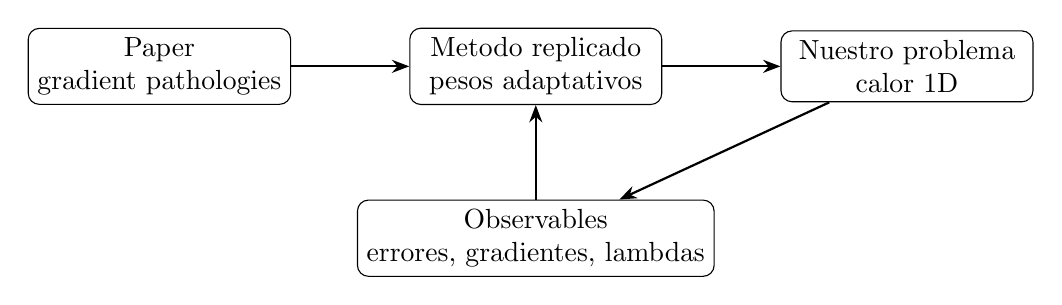
\begin{tikzpicture}[
  node distance=1.35cm,
  box/.style={draw, rounded corners, align=center, minimum width=3.2cm,
  minimum height=0.8cm},
  arrow/.style={-{Stealth[length=2.2mm]}, thick}
]
  \node[box] (paper) {Paper\\gradient pathologies};
  \node[box, right=1.5cm of paper] (method) {Metodo replicado\\pesos adaptativos};
  \node[box, right=1.5cm of method] (heat) {Nuestro problema\\calor 1D};
  \node[box, below=1.2cm of method] (obs) {Observables\\errores, gradientes, lambdas};
  \draw[arrow] (paper) -- (method);
  \draw[arrow] (method) -- (heat);
  \draw[arrow] (heat) -- (obs);
  \draw[arrow] (obs) -- (method);
\end{tikzpicture}
\caption{Trazabilidad entre el paper original y el experimento de calor 1D.}
\end{figure}

La correspondencia metodologica es:
\begin{table}[H]
\centering
\begin{tabular}{p{0.34\linewidth}p{0.55\linewidth}}
\toprule
Idea del paper & Adaptacion en el proyecto \\
\midrule
PINN clasica como baseline & M1 con
$\mathcal{L}_r+\mathcal{L}_{ic}+\mathcal{L}_{bc}$ \\
Diagnostico por gradientes separados & Histogramas y magnitudes medias por
capa para $\mathcal{L}_r$, $\mathcal{L}_{ic}$ y $\mathcal{L}_{bc}$ \\
Learning-rate annealing por gradientes & M2 con
$\lambda_{ic}$ y $\lambda_{bc}$ actualizados cada 10 iteraciones \\
Comparacion contra solucion conocida & Error relativo $L^2$ contra la solucion
analitica por separacion de variables \\
Robustez y sensibilidad & Optuna con 100 trials, validacion larga, semillas
extra y comparacion de optimizadores \\
\bottomrule
\end{tabular}
\caption{Mapa entre el nucleo metodologico del paper y nuestra implementacion.}
\end{table}

\section{Que observamos en nuestro proyecto}

La arquitectura principal final fue $[2,80,80,80,1]$ con activacion
$\tanh$, inicializacion Xavier normal, Adam, 3000 iteraciones y batch 256. Los
hiperparametros fueron seleccionados mediante 100 trials de Optuna/TPE y una
validacion larga de los mejores regimenes.

\begin{table}[H]
\centering
\begin{tabular}{lrrrr}
\toprule
Modelo & error $L^2$ rel. & tiempo [s] &
$\lambda_{ic}$ final & $\lambda_{bc}$ final \\
\midrule
M1 & 0.264333 & 208.34 & 1.00 & 1.00 \\
M2 & 0.028535 & 211.49 & 154084.83 & 251158.37 \\
\bottomrule
\end{tabular}
\caption{Resultado principal sobre calor 1D. M2 reduce el error de M1 por
un factor $9.26\times$.}
\end{table}

El resultado confirma la idea operativa del paper: el reescalado adaptativo de
los terminos de condicion inicial y borde puede cambiar de forma importante el
entrenamiento. En este problema, los pesos finales de M2 son muy grandes, lo
que indica que las estadisticas de gradiente detectaron contribuciones de
restriccion mucho mas debiles que la referencia del residuo.

\begin{figure}[H]
\centering
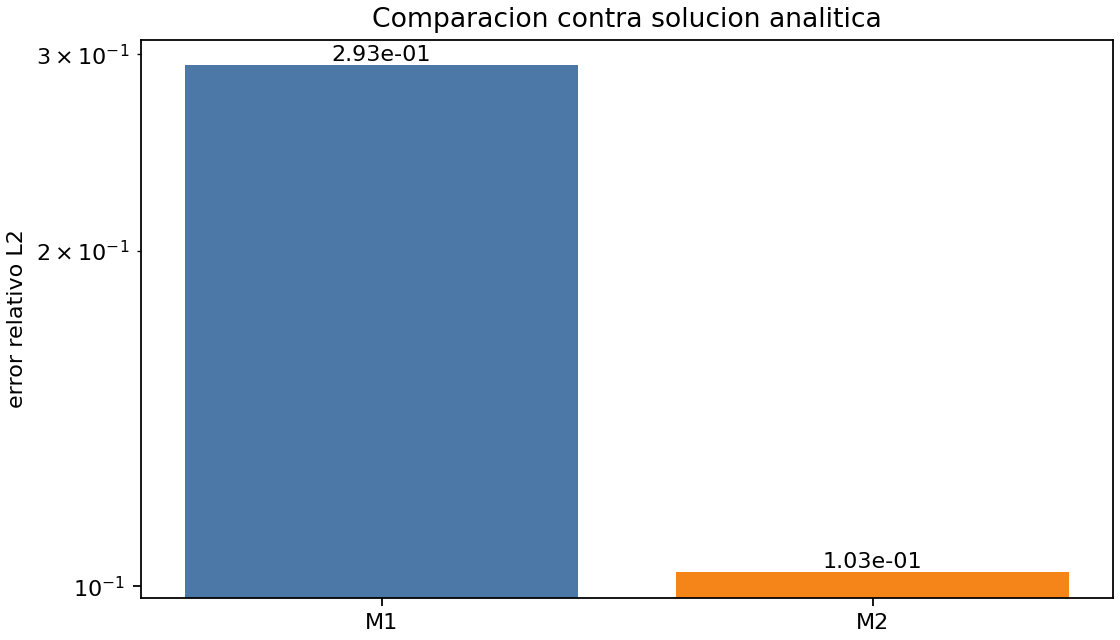
\includegraphics[width=0.72\linewidth]{outputs/comparacion_modelos.png}
\caption{Comparacion del error relativo $L^2$ entre M1 y M2.}
\end{figure}

\begin{figure}[H]
\centering
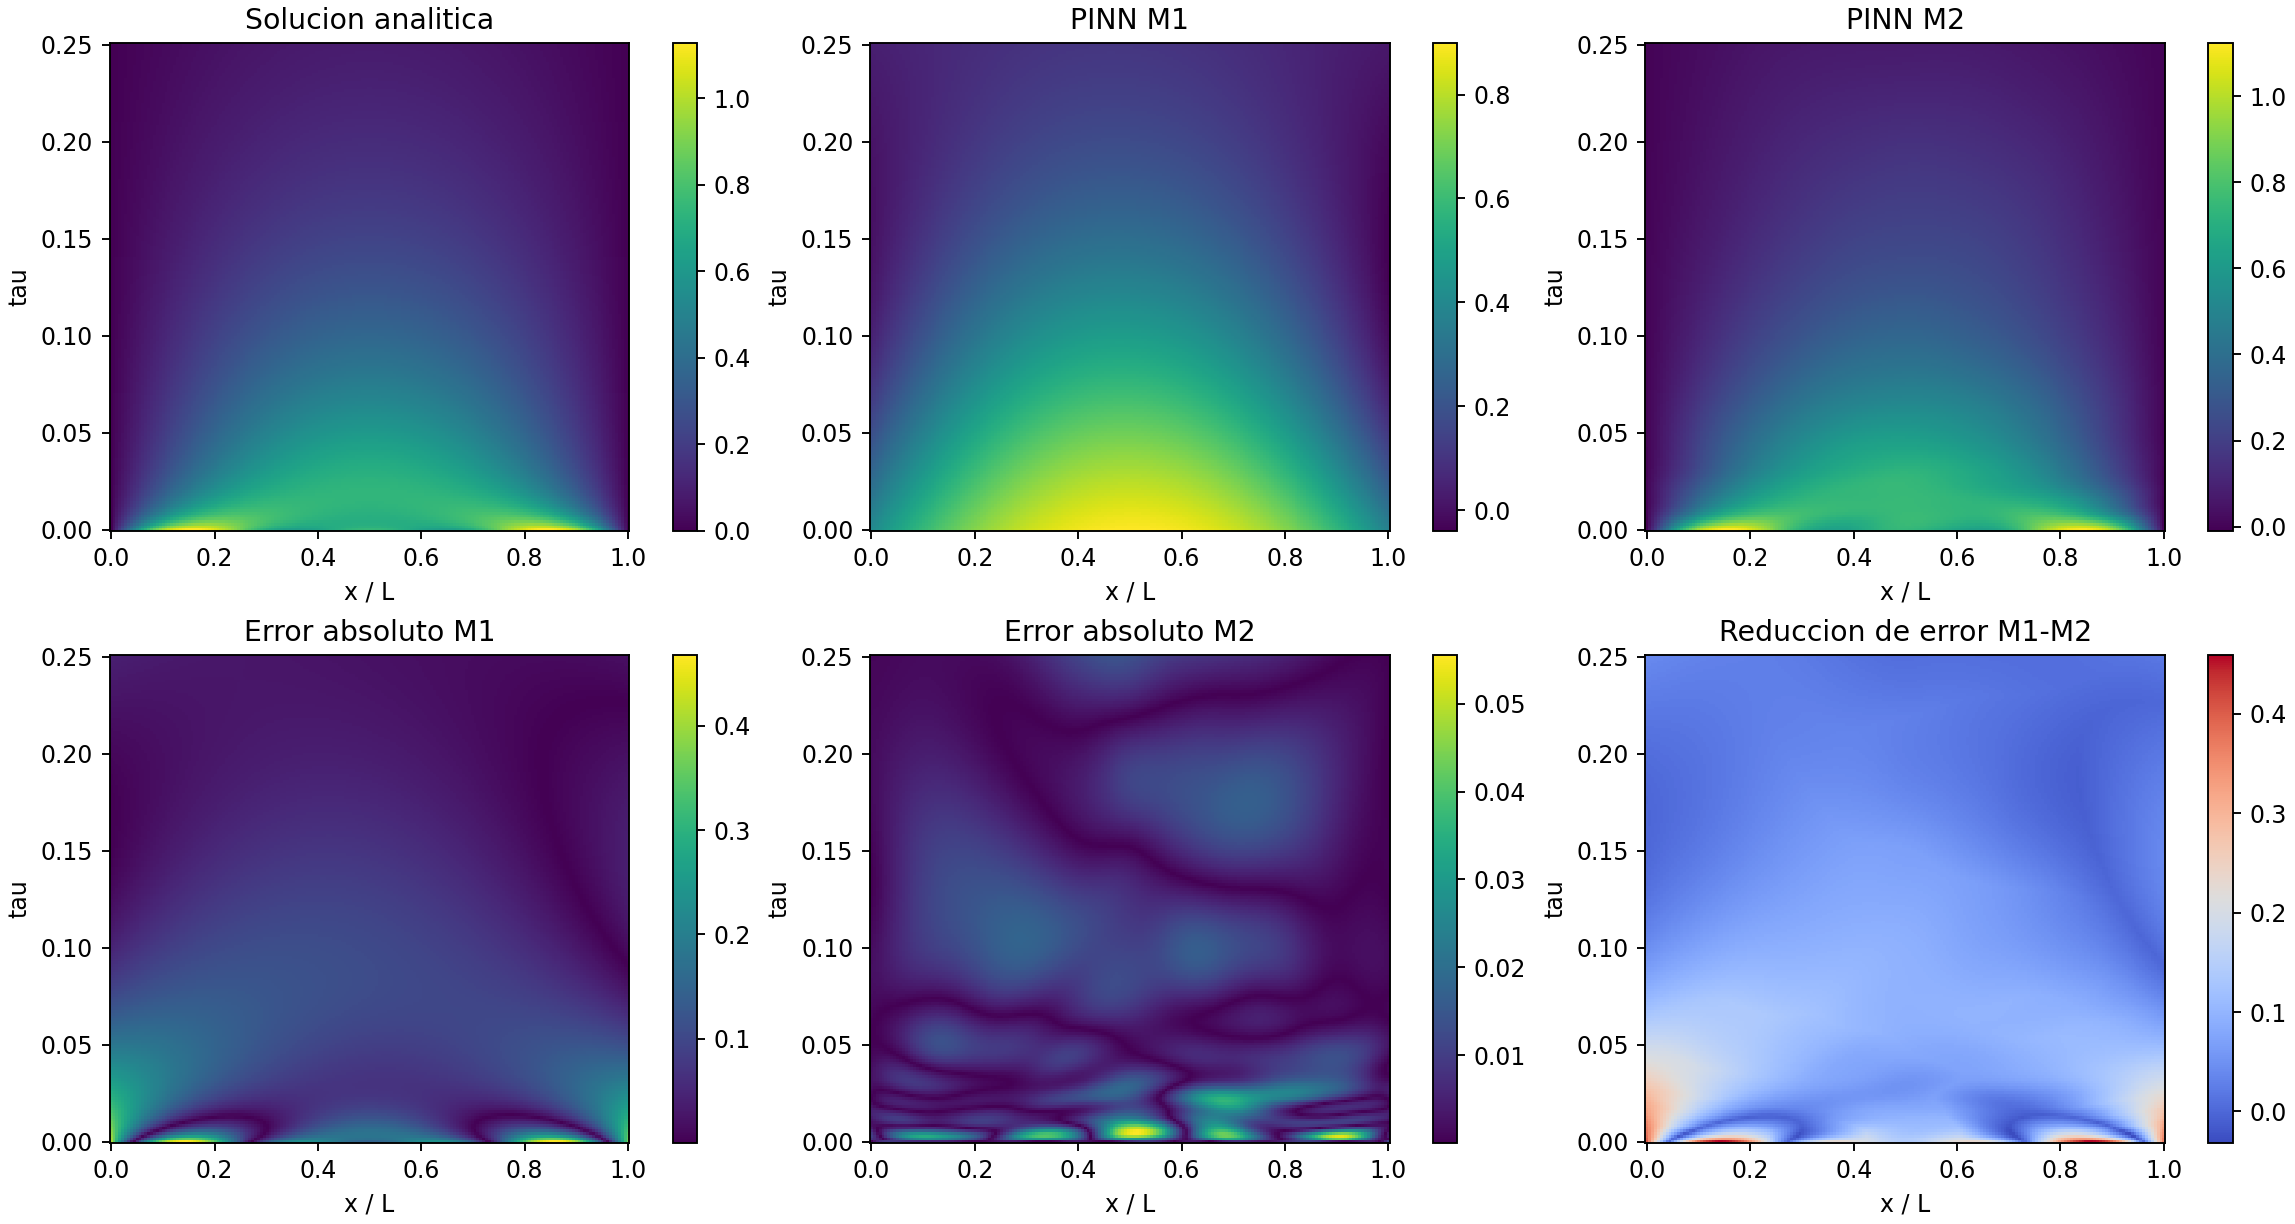
\includegraphics[width=\linewidth]{outputs/paper_comparacion_soluciones.png}
\caption{Solucion analitica, predicciones M1/M2 y mapas de error.}
\end{figure}

\begin{figure}[H]
\centering
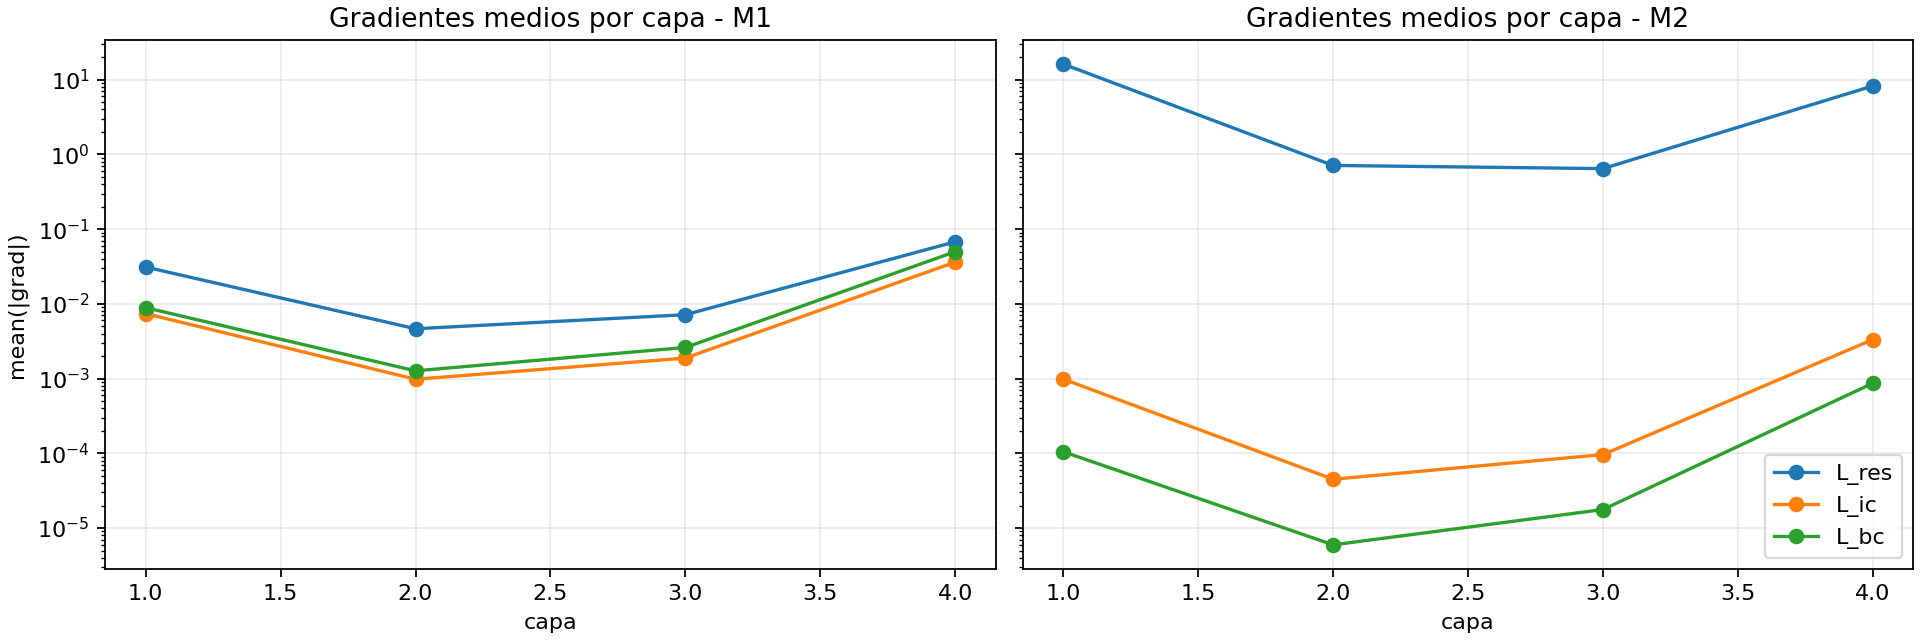
\includegraphics[width=\linewidth]{outputs/paper_balance_gradientes.png}
\caption{Diagnostico heredado del paper: magnitud media de gradientes por capa
y por termino de perdida.}
\end{figure}

\begin{figure}[H]
\centering
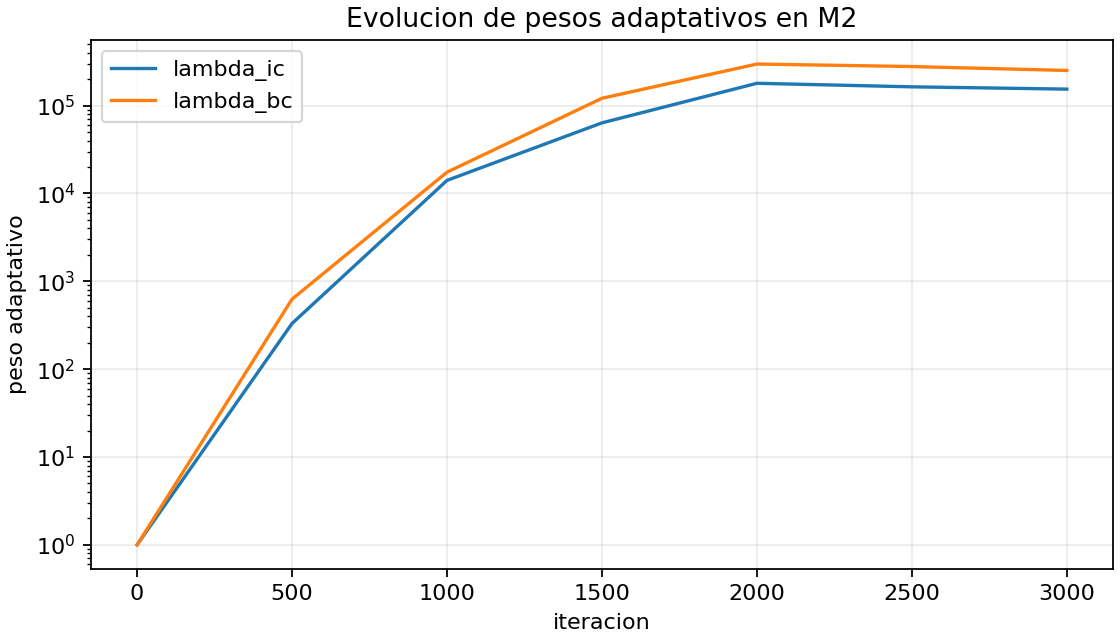
\includegraphics[width=0.78\linewidth]{outputs/paper_lambda_evolucion.png}
\caption{Evolucion de los pesos adaptativos de M2.}
\end{figure}

\section{Hiperparametros y optimizacion}

El paper advierte que no existe una receta fija de pesos $\lambda_i$ que sea
transferible entre PDEs. Por eso, ademas de implementar M2, se hizo busqueda
bayesiana de hiperparametros. El espacio explorado fue ancho de red, profundidad,
learning rate, batch y $\beta$ adaptativo. La busqueda corta eligio como mejor
trial al 91, pero la validacion larga selecciono el trial 82:
\[
  \mathrm{width}=80,\quad
  \mathrm{depth}=3,\quad
  \eta=0.0020667,\quad
  \mathrm{batch}=256,\quad
  \beta=0.96094.
\]
Esta diferencia entre el mejor trial corto y el mejor regimen validado es
coherente con el mensaje del paper: la optimizacion de PINNs debe evaluarse por
estabilidad y error final, no solo por una perdida temprana.

\begin{figure}[H]
\centering
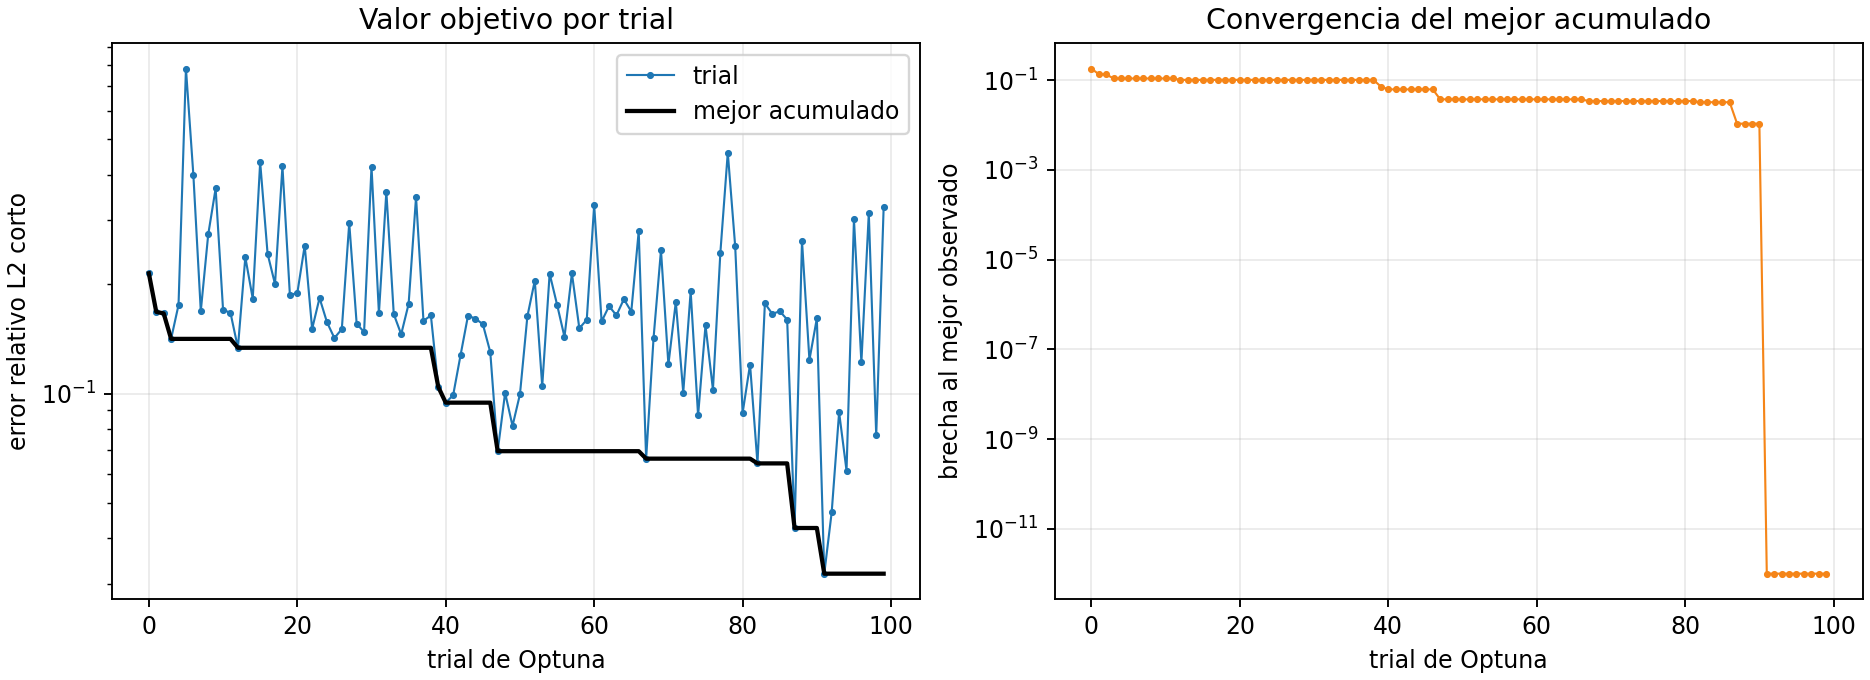
\includegraphics[width=\linewidth]{outputs/examen_bayes_convergencia.png}
\caption{Historia de Optuna: objetivo por trial y mejor acumulado.}
\end{figure}

\begin{figure}[H]
\centering
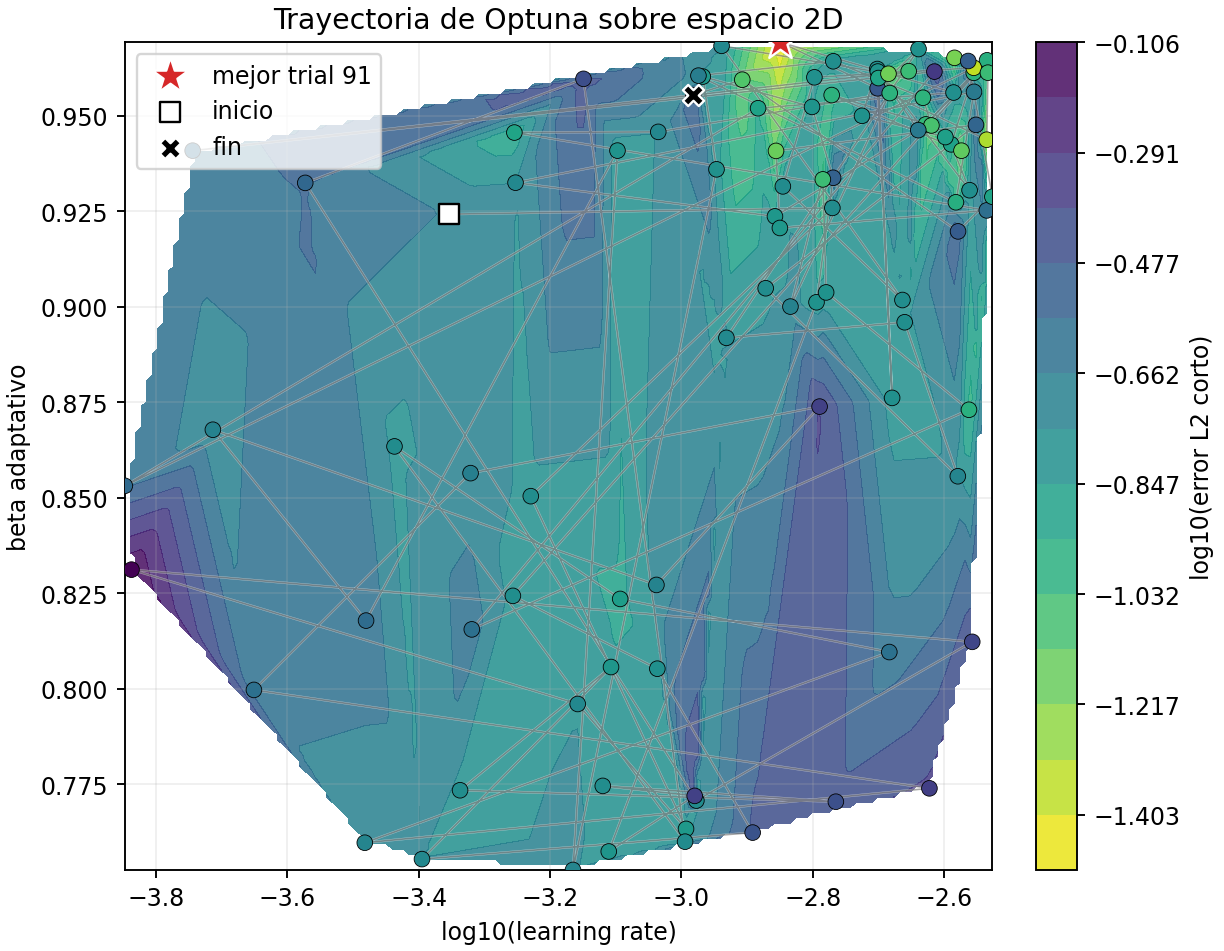
\includegraphics[width=0.78\linewidth]{outputs/examen_bayes_trayectoria_lr_beta.png}
\caption{Trayectoria de busqueda en el plano $\log_{10}(\eta)$-$\beta$.}
\end{figure}

\begin{figure}[H]
\centering
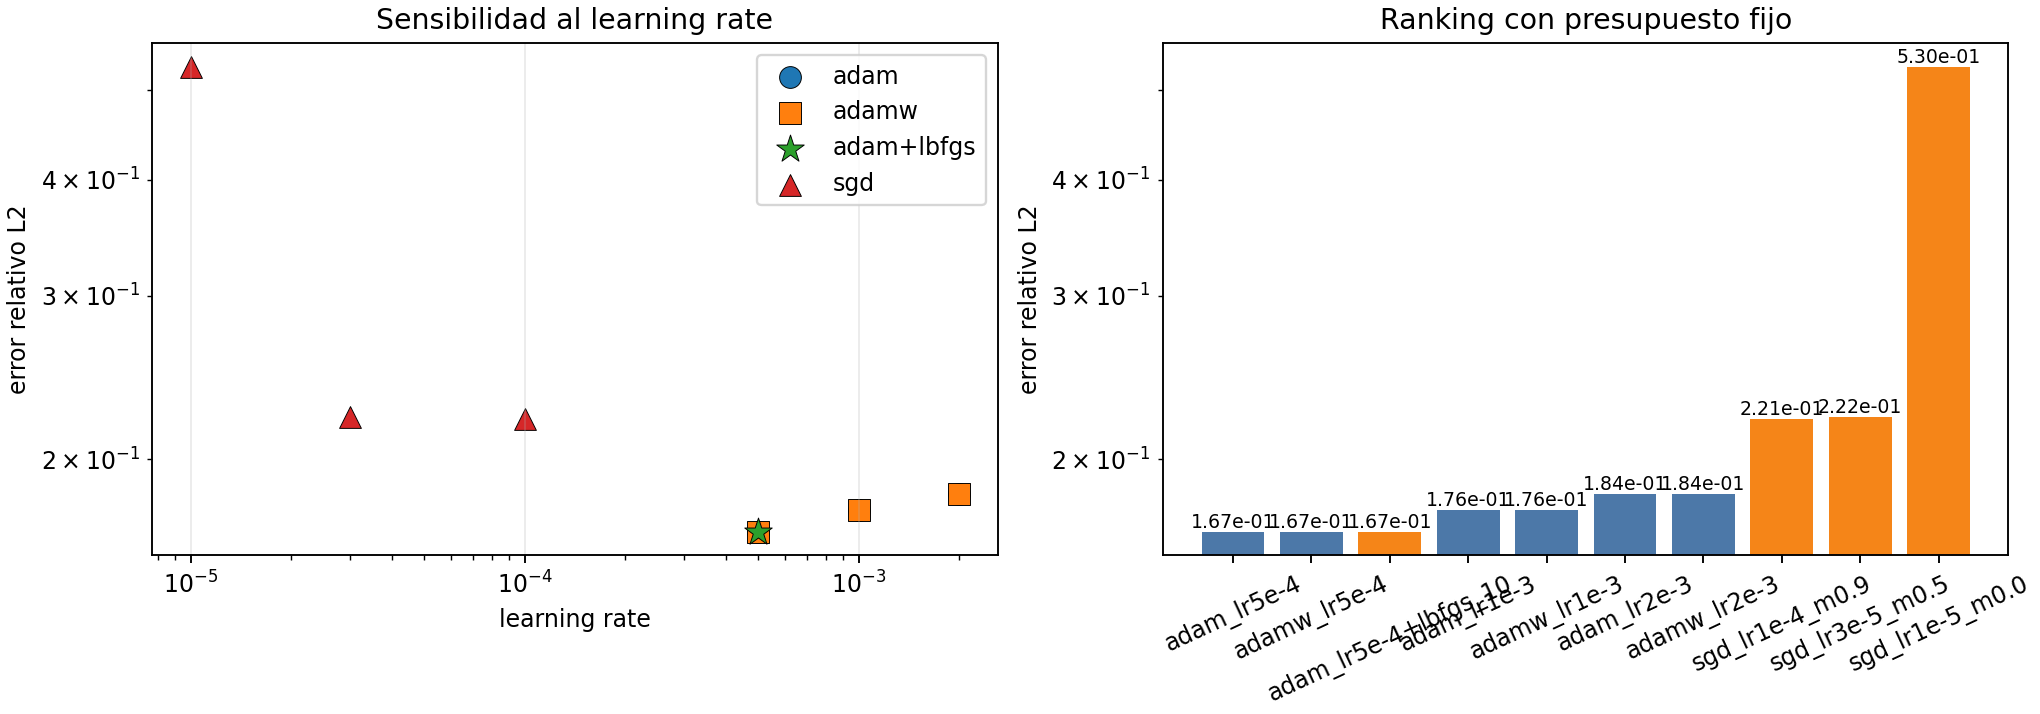
\includegraphics[width=\linewidth]{outputs/examen_optimizadores_lr_error.png}
\caption{Comparacion de optimizadores con presupuesto fijo.}
\end{figure}

\section{Lectura final}

El paper no debe leerse solamente como una propuesta de arquitectura, sino como
un analisis de optimizacion para perdidas compuestas. La leccion principal es
que, en PINNs, cumplir la PDE y cumplir las restricciones fisicas son objetivos
acoplados pero no igualmente visibles para el optimizador. Si el residuo domina
los gradientes, una red puede parecer fisicamente informada y aun asi aproximar
mal la solucion correcta.

En nuestro problema de calor 1D se observa el mismo patron metodologico:
\begin{itemize}
  \item M1 usa la formulacion clasica y alcanza un error relativo $0.2643$.
  \item M2 usa el balance adaptativo del paper y alcanza $0.0285$.
  \item La mejora no depende de cambiar la PDE ni de usar la arquitectura nueva;
  surge de modificar la geometria efectiva de la optimizacion.
  \item Los graficos de gradientes y lambdas muestran el mecanismo que explica
  la mejora, no solo el resultado numerico final.
\end{itemize}

La reproduccion es, por diseno, alternativa: no replica los ejemplos de
Helmholtz, Klein-Gordon o Navier-Stokes del paper, y no implementa M3/M4. Lo
que si replica es el nucleo tecnico que la consigna pide estudiar: diagnosticar
patologias de gradiente en PINNs y mitigarlas mediante pesos adaptativos
calculados a partir de estadisticas de gradiente.

\begin{thebibliography}{9}
\bibitem{wang2021}
S. Wang, Y. Teng, and P. Perdikaris.
\newblock Understanding and mitigating gradient flow pathologies in
physics-informed neural networks.
\newblock \emph{SIAM Journal on Scientific Computing}, 43(5):A3055--A3081,
2021.

\bibitem{repo}
Predictive Intelligence Lab.
\newblock GradientPathologiesPINNs.
\newblock \url{https://github.com/PredictiveIntelligenceLab/GradientPathologiesPINNs}.
\end{thebibliography}

\end{document}
